\documentclass[a4paper,10pt]{article}
\usepackage[top=16mm,bottom=16mm,left=18mm,right=18mm,footskip=8mm]{geometry}
\usepackage{lmodern,fontspec}
\usepackage{graphicx,xcolor,tabularx,booktabs,array,enumitem,fancyhdr,fvextra,needspace}
\setmainfont{texgyreheros-regular.otf}[
  BoldFont=texgyreheros-bold.otf, ItalicFont=texgyreheros-italic.otf,
  BoldItalicFont=texgyreheros-bolditalic.otf, Ligatures=NoCommon, RawFeature={-tlig}]
\setmonofont{lmmono10-regular.otf}
\definecolor{ink}{HTML}{182334}
\definecolor{muted}{HTML}{526079}
\definecolor{panel}{HTML}{EEF4FC}
\setlength{\parindent}{0pt}
\setlength{\parskip}{4pt}
\setlength{\tabcolsep}{4pt}
\setlist[itemize]{leftmargin=1.2em,topsep=1pt,itemsep=2pt,parsep=0pt}
\pagestyle{fancy}
\fancyhf{}
\renewcommand{\headrulewidth}{0pt}
\fancyfoot[L]{\color{muted}\fontsize{7}{9}\selectfont network24 · QOBLIB 08 · Qoro × PushQuantum 2026}
\fancyfoot[R]{\color{muted}\fontsize{7}{9}\selectfont\thepage}
\newcommand{\reportheading}[1]{\par\Needspace{3\baselineskip}\vspace{3pt}{\fontsize{11}{14}\selectfont\bfseries #1}\par\nopagebreak}
\newcommand{\reporttitle}[1]{{\fontsize{17}{21}\selectfont\bfseries #1\par}}
\newcommand{\reportnote}[1]{{\color{muted}\fontsize{8}{10}\selectfont #1\par}}
\begin{document}
\color{ink}
\fontsize{9}{11}\selectfont
\reporttitle{Network design QOBLIB 08: network24 below the best known}
\reportnote{Qoro × PushQuantum Hackathon · 21 November 2026 · network design track, instance network24 (552 binary variables)}
\noindent\colorbox{panel}{\begin{minipage}{\dimexpr\linewidth-2\fboxsep\relax}
{\fontsize{8}{10}\selectfont
\renewcommand{\arraystretch}{1.23}
\begin{tabular}{@{}>{\raggedright\arraybackslash}p{0.2565\linewidth}>{\raggedright\arraybackslash}p{0.2850\linewidth}>{\raggedright\arraybackslash}p{0.4085\linewidth}@{}}
{\fontsize{20}{24}\selectfont \textbf{657,121}} & {\fontsize{20}{24}\selectfont \textbf{\ensuremath{-}0.99\%}} & \textbf{VALID} according to the official QOBLIB Rust checker and the Python referee \texttt{qoblib\_tools.py} \\
\midrule
submission score (lower is better) & gap to the published best known, 663,688 & file: \texttt{solutions/network24.sol} \\
\end{tabular}\par
}
\end{minipage}}\par
\reportheading{The problem}
Build a directed network on 24 nodes in which every node has exactly 2 outgoing and 2 incoming links. Route all the traffic in the demand matrix; flows may split over several paths. The \textbf{score} is the load on the busiest link, in thousandths of a demand unit: the lower it is, the less congested the network. Once the topology is fixed, optimal routing is a linear program (LP) solved exactly in about 55 ms. The hard part is choosing the topology.

\reportheading{The approach: propose a topology, let the exact LP decide}
Every search follows the same loop:

\begin{itemize}
\item a \textbf{proposer} changes the current topology without ever breaking the 2-in, 2-out rule. The basic move swaps the heads of two links: (a\ensuremath{\rightarrow}b),(c\ensuremath{\rightarrow}d) \ensuremath{\Rightarrow} (a\ensuremath{\rightarrow}d),(c\ensuremath{\rightarrow}b);
\item the \textbf{exact routing LP} scores every proposal. Its dual values show which links are congested, and moves on those links are tried more often;
\item a better topology is \textbf{banked} only after a full check. Integer flows are computed, the \texttt{.sol} file is written and read back through the checker. The banked file is replaced only if the new one is valid and strictly better.
\end{itemize}
Before touching network24, the pipeline was verified on network05. From a random topology it reaches the proven optimum of 65,500, and the file passes the checker.

\reportheading{The methods, briefly}
{\fontsize{8}{10}\selectfont
\renewcommand{\arraystretch}{1.23}
\begin{tabular}{@{}>{\raggedright\arraybackslash}p{0.1615\linewidth}>{\raggedright\arraybackslash}p{0.5035\linewidth}>{\raggedright\arraybackslash}p{0.2850\linewidth}@{}}
\textbf{Method} & \textbf{How it works} & \textbf{How we used it} \\
\midrule
\textbf{Local search} & Start from a solution and change it a little, one move at a time, keeping only the changes that improve it. It stops at a \textit{local minimum}: a point where no small change helps, even though better solutions exist elsewhere. & Basic move: swap the heads of two links. It is the building block of every method below. \\
\midrule
\textbf{Simulated annealing (SA)} & Local search that sometimes accepts worse moves too, with a probability set by a \textit{temperature}. Early on the temperature is high and the search explores; then it falls and the search settles on a good solution. The name comes from annealing metals. & First submission: from 768,375 down to 684,455, then stuck. \\
\midrule
\textbf{Parallel tempering (PT)} & Several copies of the search (\textit{replicas}) run together, each at a different temperature. Hot ones explore freely, cold ones refine. Now and then two neighbouring replicas swap solutions: a good region found by a hot replica moves down to the cold ones, and a stuck cold replica gets "reheated". & 10 replicas, temperatures from 450 to 2,500. On top of that, out of 60 candidate moves only the most promising one, by a fast estimate, is scored with the LP. \\
\midrule
\textbf{Iterated local search (ILS)} & Descend to a local minimum, then apply a \textit{kick}: a few random moves that push the search out of the area. Descend again, and keep the result if it is good. Repeat with gradually stronger kicks. & 5 chains in parallel, kicks of 2 to 10 moves. \\
\midrule
\textbf{Deep step} & A variant of ILS. Instead of a random kick, take every neighbouring solution that is only slightly worse (within 1.5\%) and run a full descent from each one. A small step back often opens the way to a bigger improvement. & The step that took the score below the record: from 670,621 to 661,760. \\
\midrule
\textbf{QAOA with Divi} & A quantum optimisation algorithm. The problem is written as a QUBO, a cost over binary variables, and a circuit with tunable parameters produces samples that favour low-cost solutions. A classical optimiser tunes the parameters. & Picks 3 swaps to apply together out of 16 candidates, on 16 simulated qubits. \\
\end{tabular}\par
}
\newpage
\reportheading{How we got there}
\noindent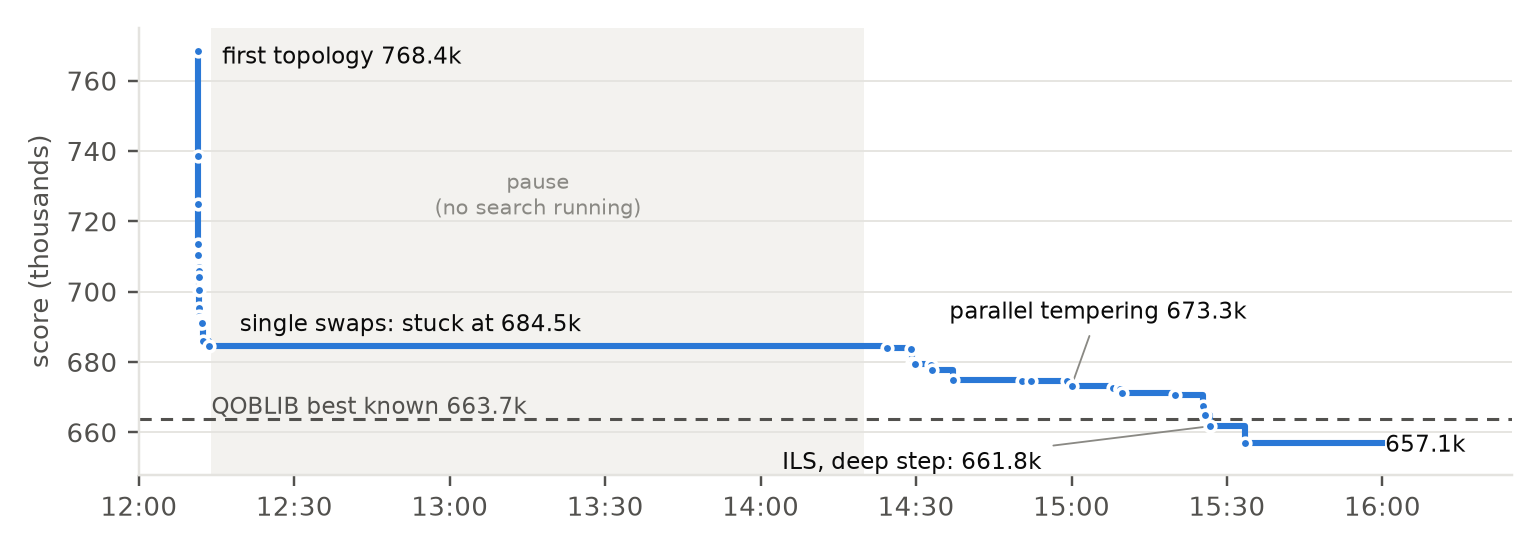
\includegraphics[width=\linewidth]{figures/network24-progress-en.png}\par
\reportnote{Best banked score on network24 over time, merging the logs of every search. Each point is a file that passed the checker.}
{\fontsize{8}{10}\selectfont
\renewcommand{\arraystretch}{1.23}
\begin{tabular}{@{}>{\raggedright\arraybackslash}p{0.2090\linewidth}>{\raggedright\arraybackslash}p{0.5320\linewidth}>{\raggedright\arraybackslash}p{0.1140\linewidth}>{\raggedright\arraybackslash}p{0.0950\linewidth}@{}}
\textbf{Phase} & \textbf{What} & \textbf{Score} & \textbf{Gap} \\
\midrule
1 · Safe submission & Topology with the most direct traffic, then simulated annealing with single swaps (2 + 10 min). Stuck at 684,455 after 12 steps. & 684,455 & +3.13\% \\
\midrule
2 · Three subagents in parallel & Parallel tempering, iterated local search (ILS) and a Divi proposer, 5 cores each, about 40 min. Parallel tempering wins. & 673,253 & +1.44\% \\
\midrule
3 · Longer parallel tempering & Same setup, 30 min, 10 workers. & 670,621 & +1.04\% \\
\midrule
4 · ILS with deep step & Restarts from 670,621 and drops below the record in about 3 minutes. & 661,760 & \ensuremath{-}0.29\% \\
\midrule
\textbf{5 · Parallel tempering from the record} & \textbf{20 min from 661,760, improvement at round 30. Verified with the Rust checker.} & \textbf{657,121} & \textbf{\ensuremath{-}0.99\%} \\
\end{tabular}\par
}
\reportheading{What worked}
\begin{itemize}
\item \textbf{Guided proposals in parallel tempering} (\texttt{network\_pt.py}). Plain parallel tempering improved nothing: cold replicas accepted 0.1–0.4\% of moves. The breakthrough was a cheap lower bound on the LP (about 0.6 ms): \ensuremath{\Sigma} demand × hop count / 48. Of K=60 generated candidates, only the one with the lowest bound goes to the LP. The median change per move drops from +25k to +8k.
\item \textbf{Deep step in ILS} (\texttt{network\_ils.py}). It got ILS out of the minima at 683,887 and 670,621, where random kicks had found nothing in 2–3 runs.
\item \textbf{Incremental LP, about 4× faster}. The HiGHS model stays open, each move edits only the links involved, and the solve restarts from the previous basis: about 15 ms instead of 55, with values identical to the original LP on 80 test topologies.
\item \textbf{More move types}: 2-swaps, swapping the roles of two nodes (up to 8 links), and reversing directed 3- or 4-node cycles. All three produced banked improvements.
\item \textbf{Independent convergence}: at 15:46 ILS found, on its own, the same 657,121 topology that parallel tempering had found at 15:33. The two files have the same SHA-256.
\end{itemize}
\reportheading{The role of Divi: a measured negative result}
The quantum proposer (\texttt{network\_divi.py}) builds a QUBO over 16 candidate swaps around the congested links. Interactions between pairs of swaps are measured exactly with the LP, and the constraint is to apply exactly 3 swaps. The QUBO is solved with QAOA p=2 on \textbf{16 qubits}, with a Dicke initial state and an XY mixer, on the local Maestro simulator. Every step is compared with other samplers on the same QUBO:

{\fontsize{8}{10}\selectfont
\renewcommand{\arraystretch}{1.23}
\begin{tabular}{@{}>{\raggedright\arraybackslash}p{0.3420\linewidth}>{\raggedright\arraybackslash}p{0.2470\linewidth}>{\raggedright\arraybackslash}p{0.1520\linewidth}>{\raggedright\arraybackslash}p{0.2090\linewidth}@{}}
\textbf{Sampler} & \textbf{Finds the best group of 3} & \textbf{In the top 5} & \textbf{Time per step} \\
\midrule
Divi QAOA-XY, 16 qubits & 44\% & 72\% & \ensuremath{\approx} 5.8 s \\
\midrule
Simulated annealing (dwave) & 29\% & 83\% & \ensuremath{\approx} 0.05 s \\
\midrule
Exact enumeration (2\textsuperscript{16} states) & 91\% & 100\% & negligible \\
\midrule
Random & 1\% & 17\% & — \\
\end{tabular}\par
}
Divi picks groups of swaps much better than chance and on par with simulated annealing, but loses to exact enumeration, which is trivial at 16 variables. Moreover, in 93 steps no group of 3 swaps improved the topology: the LP scores of every possible group, 384 per step on average, show it. \textbf{The final score comes entirely from classical search.} A program takes about 42 s at 20 qubits and about 203 s at 22, which limits how far the quantum proposer can scale.

\newpage
\reportheading{Checks and limits}
\begin{itemize}
\item The official QOBLIB Rust checker (\texttt{08-network/check}) returns \textbf{VALID} and a maximum flow of 657,121. Its controls behave as expected: the published best known is VALID at 663,688, and one of our files with a deliberately altered flow is rejected as INFEASIBLE.
\item No published solution (\texttt{network24.bst.sol}, the submissions folder) was used as a starting point or hint. Every search starts from random topologies, from the most-direct-traffic topology, or from files we banked ourselves.
\item A bug in the first ILS runs mis-scored some moves. It never affected the banked files, because the checker re-reads every file.
\item The result has not been submitted to QOBLIB yet, and \texttt{.sol} files are ignored by git: the solution exists only locally.
\end{itemize}
\reportheading{To reproduce}
\begin{Verbatim}[breaklines=true,breakanywhere=true,fontsize=\scriptsize]
NETWORK_SOL_DIR=solutions/agent_pt .venv/bin/python network_pt.py 24 --minutes 20 --replicas 10 --workers 10 --tmin 450 --tmax 2500 --banked 2 --K 60 --p-double 0.5 --p-tri 0.03 --steps 15 --seed 8
NETWORK_SOL_DIR=solutions/agent_ils .venv/bin/python network_ils.py run --chains 5 --minutes 20 --seed 700 --deep 12 --deep_tol 0.015 --kmax 8 --starts banked --sync
.venv/bin/python network_pipeline.py status
\end{Verbatim}
\reportnote{Replicas and chains run in parallel, so the same seed does not guarantee the same trajectory. Each command restarts from the file banked in its own folder.}
\end{document}
